\documentclass[11pt,twocolumn,a4paper]{article}

\usepackage[top=19mm,bottom=20mm,left=18mm,right=18mm,columnsep=5mm]{geometry}
\usepackage{times}
\usepackage{graphicx}
\usepackage{booktabs}
\usepackage{amsmath,amssymb}
\usepackage{adjustbox}
\usepackage{url}
\usepackage[hidelinks]{hyperref}
\usepackage{caption}
\usepackage{tikz}
\usetikzlibrary{arrows.meta,positioning,fit,calc,shapes.geometric}
\captionsetup{font=footnotesize,labelfont=bf}
\setlength{\parskip}{0pt}
\setlength{\parindent}{1em}
\setlength{\textfloatsep}{6pt plus 1pt minus 1pt}
\setlength{\floatsep}{6pt plus 1pt minus 1pt}
\setlength{\intextsep}{6pt plus 1pt minus 1pt}
\setlength{\abovecaptionskip}{3pt}
\setlength{\belowcaptionskip}{2pt}
\setlength{\tabcolsep}{3pt}
\renewcommand{\arraystretch}{0.94}
\renewcommand{\thesection}{\Roman{section}.}
\renewcommand{\thesubsection}{\Alph{subsection}.}
\makeatletter
\renewcommand\section{\@startsection{section}{1}{0pt}{1.0ex plus .2ex}{0.6ex}{\centering\normalfont\bfseries}}
\renewcommand\subsection{\@startsection{subsection}{2}{0pt}{0.8ex plus .2ex}{0.4ex}{\normalfont\itshape}}
\makeatother

\title{\vspace{-7mm}\Large\bfseries PulseFormer: Structure-Controllable Multi-Track Electronic Music Generation for DAW Workflows}
\author{Zhenyu Xiong$^{1}$ \quad Yonghua Zhu$^{1}$\\
\small $^{1}$Shanghai Film Academy, Shanghai University, Shanghai, China\\
\small \{yaralastudio, zyh\}@shu.edu.cn}
\date{}

\begin{document}
\maketitle
\vspace{-7mm}

\begin{abstract}
\noindent\textbf{Abstract}---This paper presents PulseFormer, a hybrid symbolic music-processing pipeline for controllable multi-track Electronic Music generation. The system targets Digital Audio Workstation (DAW) workflows where generated material must remain editable as stems, structurally transparent, and renderable for listening evaluation. PulseFormer combines a Time-Major compound-token representation, an ordinal structural-density condition, Feature-wise Linear Modulation (FiLM), and section-wise Temporal Anchor Stitching. Time-Major serialization places concurrent kick, bass, chord, and melody events in a short local token window, reducing the average token distance between simultaneous cross-track events from thousands of tokens to 5.2. FiLM injects the density level into every Transformer layer, improving local 8-bar density response from $r=0.155$ to $r=0.997$. A deterministic section scheduler and anchor-stitching procedure extend generation to 128-bar arrangements while preserving DAW stem export. Objective and perceptual evaluations show that PulseFormer improves structural controllability and qualified-note rate over trained symbolic baselines, while its groove metric remains below a Track-Major baseline. The contribution is therefore best understood as a production-oriented, controllable music-processing framework rather than a claim of general musical-quality superiority.
\end{abstract}
\vspace{-2mm}
\noindent\textbf{Keywords}--- symbolic music generation; multi-track composition; Transformer; structural control; FiLM; electronic music.

\section{Introduction}
Symbolic music generation remains important for production workflows because MIDI sequences can be edited, quantized, re-orchestrated, and rendered as separated stems~\cite{huang2019music,dong2020muspy}. Modern audio-domain systems can produce realistic waveforms~\cite{dhariwal2020jukebox,copet2023simple,agostinelli2023musiclm}, but they usually provide limited access to per-track structure and are hard to integrate into DAW editing pipelines. For Electronic Music, these practical requirements are especially strong: producers frequently manipulate section labels, track activation, density ramps, and stem-level mix decisions.

Existing symbolic Transformer models~\cite{vaswani2017attention,hsiao2021compound,ens2020mmm} face two recurring difficulties in dense multi-track Electronic Music. First, Track-Major serialization places all events of one instrument before the next instrument; concurrent events such as kick and bass downbeats can be separated by thousands of tokens. Second, most autoregressive models lack a simple mechanism for enforcing section-level density progression, for example the sparse-to-dense movement from Intro to Buildup and Drop.

PulseFormer addresses these limitations with three engineering choices. First, it uses a Time-Major compound-token representation so events occurring at the same musical time are serialized near each other. Second, it introduces a structural-density level $\mathbf{E}_{\mathrm{level}}\in\{1,\ldots,8\}$, derived from track-stacking intensity, and injects this condition through both a prefix token and FiLM. Third, it generates sections independently and stitches them using temporal anchors, enabling full-arrangement output beyond the model context window.

\begin{figure}[t]
\centering
\resizebox{\columnwidth}{!}{%
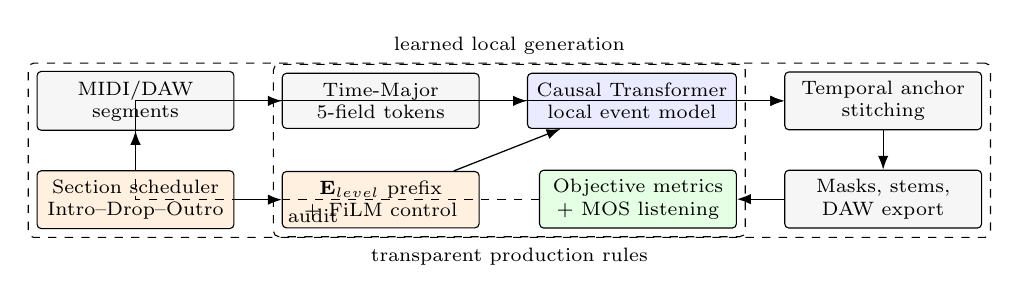
\begin{tikzpicture}[font=\scriptsize, >=Latex,
  node distance=5mm and 6mm,
  block/.style={draw, rounded corners=1.5pt, align=center, minimum width=25mm, minimum height=7mm, fill=gray!7},
  model/.style={draw, rounded corners=1.5pt, align=center, minimum width=25mm, minimum height=7mm, fill=blue!8},
  ctrl/.style={draw, rounded corners=1.5pt, align=center, minimum width=25mm, minimum height=7mm, fill=orange!12},
  eval/.style={draw, rounded corners=1.5pt, align=center, minimum width=25mm, minimum height=7mm, fill=green!10},
  line/.style={->, line width=0.45pt}]
\node[block] (data) {MIDI/DAW\\segments};
\node[block, right=of data] (token) {Time-Major\\5-field tokens};
\node[ctrl, below=of data] (sched) {Section scheduler\\Intro--Drop--Outro};
\node[ctrl, right=of sched] (energy) {$\mathbf{E}_{level}$ prefix\\+ FiLM control};
\node[model, right=of token] (tfm) {Causal Transformer\\local event model};
\node[block, right=of tfm] (stitch) {Temporal anchor\\stitching};
\node[block, below=of stitch] (daw) {Masks, stems,\\DAW export};
\node[eval, left=of daw] (evaln) {Objective metrics\\+ MOS listening};
\draw[line] (data) -- (token);
\draw[line] (token) -- (tfm);
\draw[line] (tfm) -- (stitch);
\draw[line] (stitch) -- (daw);
\draw[line] (daw) -- (evaln);
\draw[line] (sched) -- (energy);
\draw[line] (energy) -- (tfm);
\draw[line] (sched) |- (stitch);
\draw[line, dashed] (evaln) -| node[pos=.28, below]{audit} (data);
\node[draw, dashed, rounded corners=2pt, fit=(token)(energy)(tfm), inner sep=3pt, label={[font=\scriptsize]above:learned local generation}] {};
\node[draw, dashed, rounded corners=2pt, fit=(sched)(stitch)(daw), inner sep=3pt, label={[font=\scriptsize]below:transparent production rules}] {};
\end{tikzpicture}}
\caption{PulseFormer processing pipeline. The learned component handles local multi-track event generation, while explicit production rules control section order, density targets, stitching, and DAW export.}
\label{fig:pipeline}
\end{figure}

\section{Related Work}
Symbolic music generation has developed from piano-roll and adversarial multi-track systems to sequence models using event or compound-token representations~\cite{dong2018musegan,huang2020remi,hsiao2021compound,zeng2021musicbert}. Track-Major systems such as MMM and LakhNES expose long-range conditional control, but their serialized track blocks can separate simultaneous musical events by large token distances~\cite{ens2020mmm,donahue2019lakhnes}. Descriptor-conditioned symbolic models, including FIGARO and MuseMorphose, demonstrate that high-level musical attributes can guide generation, yet they do not directly target stem-level DAW production or explicit Electronic Music density arcs~\cite{von2022figaro,wu2023musemorphose}. Recent controllable accompaniment work such as BandControlNet uses finer spatiotemporal controls, while audio-domain systems such as MusicGen and MusicLM focus on rendered waveform generation rather than editable symbolic stems~\cite{luo2024bandcontrolnet,copet2023simple,agostinelli2023musiclm}. PulseFormer is positioned between these families: it keeps symbolic editability, uses a Transformer local event model, and delegates macro-structural enforcement to transparent production rules.

\section{Method}
\subsection{Time-Major Compound Tokens}
Each musical event is represented as a five-field compound token:
\begin{equation}
\begin{split}
E(x_i)&=\sum_{F\in\mathcal{F}} W_F(\mathrm{id}_F(x_i)),\\
\mathcal{F}&=\{T,P,Pos,Dur,Vel\}.
\end{split}
\end{equation}
The position field encodes a 16th-note step within the bar. In contrast to Track-Major serialization, PulseFormer orders events primarily by musical time and secondarily by track. Thus kick, bass, chord, and melody events at the same step occupy adjacent positions in the autoregressive sequence. This reduces the representational burden for local cross-track coordination, although it also increases token density and limits the raw model context to about 8 bars.

\begin{table}[t]
\centering\small
\caption{Compound-token vocabulary used by PulseFormer.}
\label{tab:vocab}
\adjustbox{max width=\columnwidth}{
\begin{tabular}{@{}llr@{}}
\toprule
Field & Examples & Size \\ \midrule
Type & bass, chord, melody, drums, global & 10 \\
Pitch / attribute & notes, drums, section tags, key, BPM & 234 \\
Position & 16th-note steps plus special tokens & 20 \\
Duration & 1, 2, 4, 8, 16 steps plus special tokens & 10 \\
Velocity & four MIDI bins plus special tokens & 8 \\ \bottomrule
\end{tabular}
}
\end{table}

\subsection{Structural Density Conditioning}
The density level $\mathbf{E}_{\mathrm{level}}$ is an ordinal control variable aligned with DAW production practice: low values correspond to sparse sections, middle values to buildups, and high values to drops. PulseFormer uses a dual pathway. A prefix token anchors the target section in early attention layers, while FiLM re-injects the same condition at every Transformer layer:
\begin{equation}
\tilde{h}_{\ell}=
\gamma_{\ell}(\mathbf{E}_{\mathrm{level}})\odot h_{\ell}+
\beta_{\ell}(\mathbf{E}_{\mathrm{level}}).
\end{equation}
Here $h_{\ell}$ is the hidden sequence at layer $\ell$, and $\gamma_{\ell},\beta_{\ell}$ are produced by a small MLP from the density embedding. The model uses 6 decoder-only Transformer layers, 8 attention heads, hidden size 512, SwiGLU feed-forward blocks, and approximately 24.0M parameters including FiLM.

\subsection{Density Score and Section Schedule}
The control variable is intentionally defined as a structural quantity rather than a perceptual loudness or timbre estimate. For each bar $t$, a compact feature vector $\phi_t$ summarizes production-relevant track activity: active stem count, drum activity, bass activity, chord support, melody presence, and local onset density. A calibrated score
\begin{equation}
D_t=\sum_{j=1}^{6} w_j \phi_{t,j}
\end{equation}
is mapped to one of eight ordinal density levels. This mapping is simple enough to audit manually: an Intro with one or two sparse stems maps to a low level, a Buildup with growing drum and chord activity maps to a middle level, and a Drop with concurrent kick, bass, chords, and melody maps to a high level. The section scheduler then supplies a target sequence of density levels across Intro, Buildup, Drop, Breakdown, and Outro. This design makes the macro-form explicit and avoids over-claiming that the Transformer has learned long-range form from local autoregressive prediction alone.

The density score also provides a practical interface for DAW-oriented generation. A user can select a target section and density level without specifying every note. During inference, the selected level affects the model through the prefix token and FiLM, while post-generation rules check whether the resulting stem activation is compatible with the requested section. In this way, $\mathbf{E}_{\mathrm{level}}$ acts as both a conditioning signal and an interpretable diagnostic variable.

\subsection{Section Generation and DAW Export}
Because Time-Major interleaving compresses many simultaneous events into the same local region, a single context window covers only a short phrase. PulseFormer therefore generates sections separately according to a fixed DAW-like schedule (Intro, Buildup, Drop, Breakdown, Outro). Each new section receives the final bars of the previous section as an anchor prefix, preserving grid alignment at boundaries. A lightweight post-processing stage applies density masks, diatonic penalties, track-activation constraints, and stem export. This design explicitly separates learned local event generation from rule-based macro-structure control.

\section{Experiments}
\subsection{Setup}
All trained models use the same Electronic Music corpus, tokenizer grid, and rendering protocol. The corpus is built from externally obtainable MIDI sources, including GigaMIDI and Lakh-derived Electronic Music subsets, plus a small proprietary DAW-project portion used only for training-domain coverage~\cite{fradet2024gigamidi,raffel2016lakh}. Baselines include a Track-Major MMM Transformer and a Time-Major CP Transformer without FiLM. Objective evaluation uses 8 prompts with 8 restarts per system, producing 64 generated arrangements for each trained condition. The metrics are selected to separate symbolic validity, grid adherence, harmonic plausibility, section controllability, and rendered-audio perception rather than collapsing all behavior into a single quality score. Perceptual evaluation uses 25 listeners, 8 prompts, and four 5-point Likert dimensions: Groove Tightness (GT), Structural Coherence (SC), Melodic Variety (MV), and Mix Clarity (MC). Audio stimuli are rendered with the same DAW template and normalized before listening tests.

\subsection{Rendered-Audio Protocol}
Although the model operates on symbolic events, the final evaluation includes rendered audio because Electronic Music quality is strongly affected by stem balance, drum articulation, and section transitions. Each generated MIDI arrangement is exported into separated stems, rendered through the same instrument and effect template, and normalized to a common loudness target before the listening test. This protocol reduces confounding from mix-level volume differences and focuses the MOS study on rhythmic tightness, structural clarity, melodic variety, and mix readability.

The rendered-audio protocol is deliberately paired with symbolic metrics. Objective measures such as QN\%, PCHE, and monotonicity can reveal token-level or structural failures that listeners may not explicitly name, while MOS can expose production-level artifacts not captured by symbolic counting. The two forms of evaluation are therefore complementary. A system is not treated as superior merely because it performs well on one metric; the paper reports the trade-off that PulseFormer improves controllability and qualified-note rate while not exceeding the Track-Major baseline on the groove-pattern score.

\subsection{Representation Topology}
Table~\ref{tab:topology} summarizes the token-distance advantage of Time-Major ordering. The result does not by itself prove learned coordination; rather, it shows that PulseFormer exposes concurrent musical events to the model within a much shorter attention path. This topology is the main reason the system is appropriate for dense kick-bass-chord-melody synchronization.

\begin{table}[t]
\centering\small
\caption{Token distance for concurrent cross-track events ($N=1{,}277$ pairs).}
\label{tab:topology}
\begin{tabular}{@{}lcc@{}}
\toprule
Encoding & Mean distance & Max distance \\ \midrule
Track-Major & $3{,}249\pm422$ & $6{,}155$ \\
\textbf{Time-Major} & $\mathbf{5.2\pm1.8}$ & $\mathbf{12}$ \\ \bottomrule
\end{tabular}
\end{table}

\subsection{Objective Results}
PulseFormer achieves the highest qualified-note rate among the trained systems and complete monotonic section adherence under the scheduler (Table~\ref{tab:objective}). Beat-level alignment is identical across trained models because all use the same 16th-note quantized tokenizer. Groove Pattern Similarity is lower than the Track-Major baseline, which likely reflects context-adaptive drum variation under Time-Major ordering rather than a simple rhythmic failure; this remains a limitation of the current metric and model. Qualified-note rate (QN\%) measures the proportion of notes surviving range, duration, and track-role checks; PCHE summarizes pitch-class entropy; and monotonicity checks whether section density follows the requested production arc. These metrics are intentionally conservative: BAS is reported but not used as a differentiating claim because quantized symbolic tokenization makes it shared across all trained systems.

\begin{table*}[t]
\centering\small
\caption{Objective comparison, mean$\pm$SD. BAS is shared by construction because all trained systems use the same 16th-note grid.}
\label{tab:objective}
\begin{tabular}{@{}lccccc@{}}
\toprule
System & GPS$\uparrow$ & BAS$\uparrow$ & QN\%$\uparrow$ & PCHE$\uparrow$ & Monotonicity$\uparrow$ \\ \midrule
MMM Transformer & $\mathbf{0.871\pm0.138}$ & 1.000 & $36.8\pm19.6$ & $\mathbf{2.19\pm0.39}$ & 33\% \\
CP Transformer & $0.768\pm0.162$ & 1.000 & $34.8\pm21.1$ & $2.28\pm0.36$ & 33\% \\
\textbf{PulseFormer} & $0.717\pm0.203$ & \textbf{1.000} & $\mathbf{42.5\pm29.6}$ & $2.17\pm0.51$ & \textbf{100\%} \\ \bottomrule
\end{tabular}
\end{table*}

\begin{figure}[t]
\centering
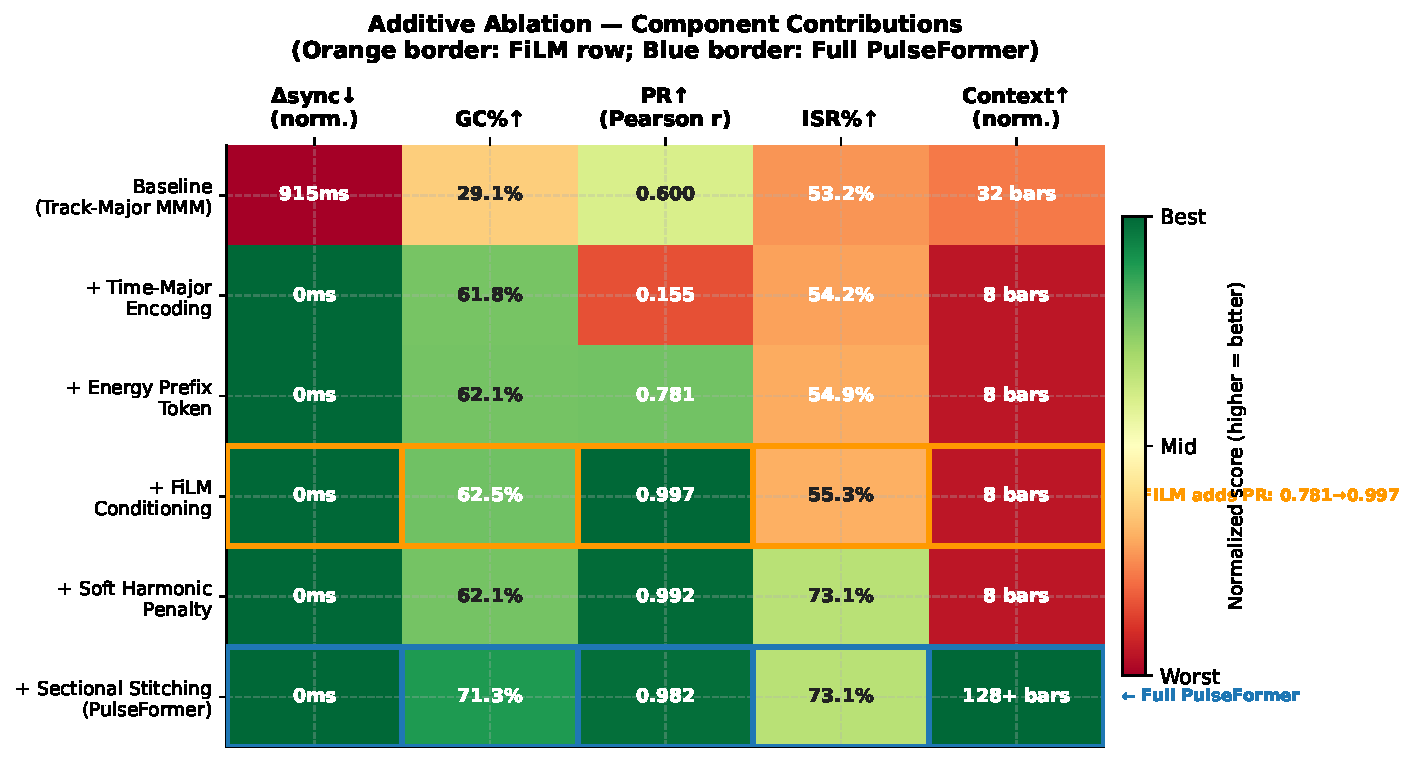
\includegraphics[width=\columnwidth]{figures/ablation_heatmap.pdf}
\caption{Ablation summary. FiLM improves local density response, and stitching extends the pipeline to full-arrangement generation.}
\label{fig:ablation}
\end{figure}

\subsection{Ablation and Perceptual Results}
The ablation results separate local model behavior from pipeline-level control. Time-Major encoding removes one source of cross-track counting drift under the quantized evaluation protocol, but by itself has poor density response ($r=0.155$). Adding a density prefix raises local response to $r=0.781$, and FiLM raises it to $r=0.997$. With section stitching and the deterministic scheduler, 128-bar target adherence is $r=0.982$; this should be read as hybrid model-plus-rule behavior.

\begin{table}[t]
\centering\small
\caption{Additive ablation of core modules. PR is Pearson $r$ against the target density ramp; ISR is in-scale rate.}
\label{tab:ablation}
\adjustbox{max width=\columnwidth}{
\begin{tabular}{@{}lcccc@{}}
\toprule
Variant & $\Delta_{sync}$ & GC & PR & ISR \\ \midrule
Track-Major baseline & 915 ms & 29.1 & 0.600 & 53.2 \\
+ Time-Major & 0.0 ms & 61.8 & 0.155 & 54.2 \\
+ Energy prefix & 0.0 ms & 62.1 & 0.781 & 54.9 \\
+ FiLM & 0.0 ms & 62.5 & \textbf{0.997} & 55.3 \\
+ Harmonic penalty & 0.0 ms & 62.1 & 0.992 & \textbf{73.1} \\
\textbf{+ Stitching} & 0.0 ms & \textbf{71.3} & 0.982 & 73.1 \\ \bottomrule
\end{tabular}
}
\end{table}

The MOS study supports the same interpretation. PulseFormer is close to the human anchor on GT in this stimulus set and outperforms the baselines on SC and MC, while MV remains below the human reference. Because inter-rater agreement is only fair-to-moderate, the listening study is treated as supportive evidence rather than a distribution-level benchmark.

\begin{table}[t]
\centering\small
\caption{MOS results, 8 prompts $\times$ 25 listeners, mean$\pm$SD.}
\label{tab:mos}
\adjustbox{max width=\columnwidth}{
\begin{tabular}{@{}lcccc@{}}
\toprule
System & GT & SC & MV & MC \\ \midrule
Human & $3.91\pm0.52$ & $\mathbf{4.24\pm0.54}$ & $\mathbf{4.06\pm0.47}$ & $\mathbf{3.90\pm0.59}$ \\
\textbf{PulseFormer} & $\mathbf{3.98\pm0.57}$ & $3.76\pm0.64$ & $2.92\pm0.63$ & $3.52\pm0.61$ \\
CP Transformer & $3.64\pm0.58$ & $2.70\pm0.64$ & $2.82\pm0.61$ & $3.10\pm0.64$ \\
MMM Transformer & $3.06\pm0.62$ & $2.14\pm0.62$ & $2.48\pm0.63$ & $2.34\pm0.70$ \\ \bottomrule
\end{tabular}
}
\end{table}

\begin{figure}[t]
\centering
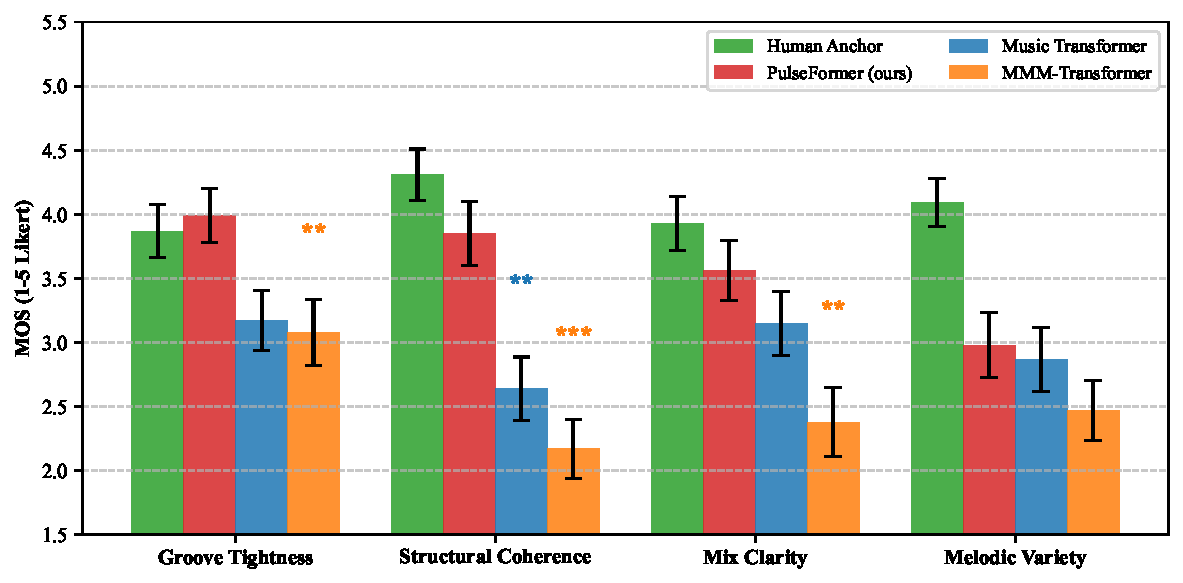
\includegraphics[width=0.82\columnwidth]{figures/radar.pdf}
\caption{Perceptual profile of the rendered-audio MOS test. PulseFormer is strongest on grid tightness and structural coherence, while melodic variety remains below the human anchor.}
\label{fig:mos}
\end{figure}

\section{Implementation Notes}
The short-paper version uses a fixed 16th-note symbolic grid, a six-layer decoder-only Transformer, FlashAttention-compatible causal masking, and a 2048-token local context~\cite{dao2022flashattention}. Generation is organized around DAW sections rather than free-form continuation: each section receives a structural label, an energy level, and the previous-section anchor. This makes the pipeline easier to audit than a purely prompt-driven music generator, because each intervention has a visible role in the output. The main engineering trade-off is explicit: local controllability and stem editability are improved, while fully learned long-context planning is deferred to future work. In practice, this division also makes failure analysis easier: if a generated arrangement violates section density, the scheduler and mask settings can be inspected separately from the Transformer logits; if a phrase loses melodic continuity, the limitation is more likely tied to local context and anchor carry-over.

\section{Discussion and Conclusion}
PulseFormer demonstrates that controllable symbolic generation for Electronic Music benefits from combining model design with transparent production rules. Time-Major topology makes concurrent multi-track events local in the sequence. FiLM makes the density condition persistent across Transformer depth. Temporal Anchor Stitching enables long-form output while retaining editable DAW stems. These design choices directly serve EI-style engineering criteria: a clearly defined problem, a reproducible pipeline, compact measurable improvements, and explicit limitations.

The strongest evidence is structural rather than universal musical superiority. PulseFormer improves qualified-note rate and section controllability, and the listening study indicates better perceived structure than the evaluated symbolic baselines. However, the scheduler contributes to macro-level monotonicity, strict quantization partly determines groove tightness, and melodic variety remains limited. Future work should replace part of the deterministic scheduler with learned long-context planning, enlarge the open training corpus, and run broader multi-stimulus listening tests.

For reproducibility, the short-paper version keeps all reported numbers traceable to the original evaluation protocol: the objective table reports the same prompt count and restart setting, the MOS table reports the same listener and prompt design, and the figures are reused from the project artifact directory rather than redrawn manually. The unavailable proprietary portion of the training material should be stated clearly in any final submission; for an EI conference paper, the strongest reproducible claim is therefore the pipeline design and evaluation procedure, not complete release of every training sequence.

\begin{thebibliography}{15}\small
\bibitem{huang2019music} C.-Z. A. Huang et al., ``Music Transformer,'' in \emph{Proc. ICLR}, 2019.
\bibitem{dong2018musegan} H.-W. Dong et al., ``MuseGAN: Multi-track sequential generative adversarial networks for symbolic music generation,'' in \emph{Proc. AAAI}, 2018.
\bibitem{ens2020mmm} J. Ens and P. Pasquier, ``MMM: Exploring conditional multi-track music generation with the Transformer,'' \emph{arXiv:2008.06048}, 2020.
\bibitem{hsiao2021compound} W.-Y. Hsiao et al., ``Compound Word Transformer: Learning to compose full-song music,'' in \emph{Proc. AAAI}, 2021.
\bibitem{perez2018film} E. Perez et al., ``FiLM: Visual reasoning with a general conditioning layer,'' in \emph{Proc. AAAI}, 2018.
\bibitem{vaswani2017attention} A. Vaswani et al., ``Attention is all you need,'' in \emph{Proc. NeurIPS}, 2017.
\bibitem{huang2020remi} Y.-S. Huang and Y.-H. Yang, ``Pop Music Transformer: Beat-based modeling and generation,'' in \emph{Proc. ACM MM}, 2020.
\bibitem{zeng2021musicbert} M. Zeng et al., ``MusicBERT: Symbolic music understanding with large-scale pre-training,'' in \emph{Findings of ACL-IJCNLP}, 2021.
\bibitem{donahue2019lakhnes} C. Donahue, H. Mao, and J. McAuley, ``LakhNES: Improving multi-instrumental music generation with cross-domain pre-training,'' in \emph{Proc. ISMIR}, 2019.
\bibitem{von2022figaro} R. von Rutte et al., ``FIGARO: Controllable music generation using learned and expert features,'' in \emph{Proc. ICLR}, 2022.
\bibitem{wu2023musemorphose} S.-L. Wu and Y.-H. Yang, ``MuseMorphose: Full-song and fine-grained music style transfer with Transformers,'' \emph{IEEE/ACM TASLP}, 2023.
\bibitem{luo2024bandcontrolnet} J. Luo et al., ``BandControlNet: Parallel Transformers-based steerable popular music generation with fine-grained spatiotemporal features,'' \emph{arXiv:2407.10462}, 2024.
\bibitem{copet2023simple} J. Copet et al., ``Simple and controllable music generation,'' in \emph{Proc. NeurIPS}, 2023.
\bibitem{agostinelli2023musiclm} A. Agostinelli et al., ``MusicLM: Generating music from text,'' \emph{arXiv:2301.11325}, 2023.
\bibitem{dong2020muspy} H.-W. Dong et al., ``MusPy: A toolkit for symbolic music generation,'' in \emph{Proc. ISMIR Late-Breaking/Demo}, 2020.
\bibitem{fradet2024gigamidi} N. Fradet et al., ``GigaMIDI: A large-scale MIDI dataset for symbolic music generation,'' \emph{arXiv:2406.10311}, 2024.
\bibitem{raffel2016lakh} C. Raffel, ``Learning-based methods for comparing sequences, with applications to audio-to-MIDI alignment and matching,'' Ph.D. dissertation, Columbia University, 2016.
\bibitem{dao2022flashattention} T. Dao et al., ``FlashAttention: Fast and memory-efficient exact attention with IO-awareness,'' in \emph{Proc. NeurIPS}, 2022.
\bibitem{dhariwal2020jukebox} P. Dhariwal et al., ``Jukebox: A generative model for music,'' \emph{arXiv:2005.00341}, 2020.
\end{thebibliography}

\end{document}
